\documentclass[conference]{IEEEtran}
\IEEEoverridecommandlockouts
% The preceding line is only needed to identify funding in the first footnote. If that is unneeded, please comment it out.
\usepackage{cite}
\usepackage{amsmath,amssymb,amsfonts}
\usepackage{algorithmic}
\usepackage{graphicx}
\usepackage{textcomp}
\usepackage{xcolor}
\def\BibTeX{{\rm B\kern-.05em{\sc i\kern-.025em b}\kern-.08em
    T\kern-.1667em\lower.7ex\hbox{E}\kern-.125emX}}


% % Vector
% \newcommand{\vect}[1]{\vec{#1}}
% \renewcommand{\vec}[1]{\bm{#1}}
% % Matrix
% \newcommand{\mat}[1]{\bm{\mathrm{#1}}}



\begin{document}

\title{Towards Predictive Maintenance: an Edge-based Vibration Monitoring System in Practice}





\author{\IEEEauthorblockN{1\textsuperscript{st} Victor Lorhan Loiola Costa}
\IEEEauthorblockA{\textit{dept. name of organization (of Aff.)} \\
\textit{name of organization (of Aff.)}\\
City, Country \\
email address or ORCID}
\and
\IEEEauthorblockN{2\textsuperscript{nd} Given Name Surname}
\IEEEauthorblockA{\textit{dept. name of organization (of Aff.)} \\
\textit{name of organization (of Aff.)}\\
City, Country \\
email address or ORCID}
\and
\IEEEauthorblockN{3\textsuperscript{rd} Given Name Surname}
\IEEEauthorblockA{\textit{dept. name of organization (of Aff.)} \\
\textit{name of organization (of Aff.)}\\
City, Country \\
email address or ORCID}
\and
\IEEEauthorblockN{4\textsuperscript{th} Given Name Surname}
\IEEEauthorblockA{\textit{dept. name of organization (of Aff.)} \\
\textit{name of organization (of Aff.)}\\
City, Country \\
email address or ORCID}
\and
\IEEEauthorblockN{5\textsuperscript{th} Given Name Surname}
\IEEEauthorblockA{\textit{dept. name of organization (of Aff.)} \\
\textit{name of organization (of Aff.)}\\
City, Country \\
email address or ORCID}
\and
\IEEEauthorblockN{6\textsuperscript{th} Given Name Surname}
\IEEEauthorblockA{\textit{dept. name of organization (of Aff.)} \\
\textit{name of organization (of Aff.)}\\
City, Country \\
email address or ORCID}
}

\maketitle

\begin{abstract}
Due to the high acquisition and operation cost of industrial machinery, the cost-effectiveness is highly influenced by the quality and continuity of their production. In this context, Predictive Maintenance emerges as a maintenance strategy aiming to maximize uptime by constantly monitoring a quantity related to the machine's health, such as vibration patterns, in order to perform maintenance stops only when strictly required. The implementation of this strategy, however, faces multiple challenges. One of them is related to the design, installation and operation of the sensoring systems required, which are subjected to budget constraints and also technical constraints such as sensor battery lifetime. Another challenge is given by the intelligence required for analysing real-world data generated within uncontrolled industrial environments and producing a machinery health indicator from it. This work illustrates a vibration monitoring system currently operating in a textile manufacturing machine; proposes a versatile Anomaly-Detection-based procedure for the analysis the real-world data produced by such systems and extraction of a machine health indicator from it; and also proposes an extension to the system in order to adapt it to the connectivity requirements set by the current context of Industry 4.0.
\end{abstract}



\begin{IEEEkeywords}
Predictive Maintenance, Anomaly Detection, Vibration Monitoring
\end{IEEEkeywords}

\section{Introduction}

\subsection{The Way to Predictive Maintenance}

Today’s industrial machinery are usually capital-intensive. Hence, keeping such equipment in optimal operating condition with the highest availability, performance, and quality is viewed as a crucial part of ensuring the return on investment in the acquisition and operation. In this context, machine maintenance, a vital aspect of the Overall Equipment Effectiveness (OEE), ensures that a facility satisfies production schedules, minimizes machinery downtime, and prevents potential accidents in workplaces (\cite{chong2015}, \cite{b1}). 

Different maintenance strategies are proposed as the complexity of machinery and their working environment increase over time. In general, they can be divided into \cite{b1}:

\begin{enumerate}
	\item reactive maintenance: performing maintenance when an issue is presented
	\item preventive maintenance: performing maintenance due to failure experience accumulated by machine producers and operators
	\item predictive maintenance: performing maintenance based on the evaluation of data collected from equipped sensors and other sources
\end{enumerate}

In comparison with reactive and preventive maintenance, predictive maintenance detours unnecessary maintenance stops and unscheduled machine downtime since the machine is constantly monitored, and the maintenance will solely be performed when failure is imminent.

\subsection{Associated challenges}
\label{sec_associated_challenges}

Developing predictive maintenance concepts is encountered a wide range of challenges, such as cost, operational variability, and data privacy. First, as predictive maintenance is based on machine monitoring data collected from different sensors, the cost of the acquisition and installation of sensors is involved and can vary according to the complexity of the data model applied. Besides, individual machines produced as the same type might operate differently under different conditions. Hence, ensuring the general availability of the data-based model developed for a certain machine type evolves into another problem. Furthermore, accompanied by the increased complexity of methods and the quality of data flow, the requirements for hardware to process are restricted. Finally, data always implicates some sensitive information about production and business. Preventing data tampering and leakage is considered as well.

\subsection{Industry 4.0 - Enabling Predictive Maintenance}

In the current context of Industry 4.0, large amounts of devices are internetworked. The term Internet of Things (IoT) emerges as the amalgam of software techniques, communication technologies, and individual devices that constitute these networks which, despite the name, may or may not be connected to the internet.

The emerging chip technology facilitates the development of edge devices which, compared with cloud devices, provide the following advantages: $1)$ reduced latency, $2)$ improved security, $3)$ reduced infrastructure cost, $4)$ improved reliability, and $5)$ large autonomy for battery-powered devices. The combination of edge devices and predictive maintenance covers the challenges mentioned above.


\subsection{Our contribution}

This paper illustrates an edge-based vibration monitoring system currently operating in a textile manufacturing machine and proposes a versatile anomaly-detection-based procedure for the analysis of real-world data and extraction of machine health status, considering the battery life of sensors.

The remaining part of the paper is structured as follows: Section \ref{sec_related_work} provides an overview of the related work regarding predictive maintenance concepts for vibration analysis. In Section \ref{sec_concept}, we propose our concept for data analysis techniques. The implementation details are presented in Section \ref{sec_implementation}. We highlight the results of the data analysis and indicate our discussion in Section \ref{sec_results_discussion}. Consequently, the paper is concluded in Section \ref{sec_conclusion}.



\section{Related work}
\label{sec_related_work}

Examples of sucessfull applications of the predictive maintenance approach for a wide range of industries can be seen in, for example, \cite{adebiyi}, \cite{alnajjar} and \cite{doyleek}.

An exploration of the challanges and strategies involved in achieving sucess in the implementation of predictive maintenance is found in \cite{carnero2006evaluation}.

The potential presented by vibration analysis to be developed into PM solutions is presented in \cite{b1}, which also discusses in detail the fundamentals required for the development of physics-based solutions.

Data-based approaches, which shift the focus of the intelligence required from expert-knowledge to historical data, are exploited in numerous studies. 


For example, \cite{wu2017remaining} and \cite{li2020lifelong} present vibration-based PM methods with labeled data obtained from experiments in controlled conditions. Another approach is given in \cite{cui2018anomaly}, which presents a condition monitoring approach for wind power equipment in field operating conditions, with a modelling which also uses labeled data and a type of machine which works with low operational variability.





% ===============================================================
% ===============================================================
% ===============================================================
\section{Concept - Data analysis techniques}
\label{sec_concept}

The vibration monitoring solution proposed in this work employs a range of techniques within the realm of data and signal analysis. This Section is dedicated to summarizing them, see Figure \ref{techniques_overview}. 

First, in Section \ref{sec_vibration_analysis}, we present a discussion about the field of machine vibration analysis, which is required in order to gain insights into how to interpret the vibration signals and learn which of its features can be correlated to the machine's condition. In Section \ref{sec_signal_processing} we present an overview of the implemented signal processing techniques to extract the desired features from the vibration signals. In Section \ref{sec_clustering} we discuss the data clustering techniques used to identify and segregate the potentialy multiple operational modes presented by the machine under study. Finaly, in Section \ref{sec_anomaly_detection} we explore the Anomaly Detection concept and discuss about how to use the multi-variate Gaussian distribution to implement Anomaly Detection in the scenario at hand.

\begin{figure}[htbp]
\centerline{\includegraphics[width=\columnwidth]{graphics/techniques/techniques_block.pdf}}
\caption{Overview of the techniques employed in the data analysis.}
\label{techniques_overview}
\end{figure}



% ===============================================================
\subsection{Vibration Analysis}
\label{sec_vibration_analysis}
% RMS numerical value of total vibration. Speed is always important. Induction motors. Frequency Analysis: helps identifying source of problem.
% Which features are important.



In the context of PM of rotating machinery, vibration analysis is widely considered the single most important technique available \cite{b1}. It provides a robust method for monitoring the general health of an equipment by indicating the onset and/or presence of many fault mechanisms, including \cite{b1}:

\begin{itemize}
    \item Shaft misalignment
    \item Rotor unbalance
    \item Mechanical looseness
    \item Bear and gearing damage/degradation
    \item Inadequate reassembly after maintenance
\end{itemize}

In order to carry out this kind of analysis, the process starts with the aquisition of vibration signals of the machine under test by means of a vibration transducer. Then, the vibration waveforms can be analysed by multiple techniques.

In the simplest approach, we consider the vibration of rotating machinery is generally to be avoided. Although it is physically impossible to have a rotating machine that does not produce vibration, the intensity of this vibration should be kept within acceptable levels dictated by the mechanical structure of the machine and the environment where it is located.

This approach gives little indication of what the root cause of an underlying problem might be. A more sophisticated approach is the frequency analysis of the vibration waveform. The decomposition of the vibration signal into its frequency components is explained in more detail in Section \ref{sec_signal_processing}. Once the frequency components are obtained, one can associate the amplitudes over the frequency spectra to the frequencies where mechanical problems such as the ones listed in this section are expected to appear. Also, while the frequency indicates the source of the vibration, the amplitude indicates the severity of the problem.

The process of associating specific mechanical problems to a machine’s vibration frequency spectra involves knowledge of a plethora of characteristics such as bearing and gear geometry and materials, type of grease, maintenance history and so on \cite{b1}.

A basic characteristic is the rotating speed of the motors. A very common type of motor used in industrial rotating machinery is the four-pole three-phase electric induction motor \cite{b2}. This type of machine presents a mechanical rotation slightly less then half that of its alternate current electric supply. Thus, for a motor being operated with a 60 Hz alternate current input, we expect a peak around 30Hz for rotating machinery with such motors. Thus, for the case of machine speed control by means of the motor, the position where the peak around 30Hz appears is directly related to the speed the machine is operated at. This is particularly meaningful, as the machine’s speed can exert a high influence on its vibration pattern. Hence, the vibration analysis should take the machine’s speed into account \cite{b3}.


% ===============================================================
\subsection{Signal Processing}
\label{sec_signal_processing}

As exposed in Section \ref{sec_vibration_analysis}, the following characteristics of the vibration signal are of particular interest for an estimation of the machine's condition:

\begin{itemize}
	\item Machine's speed
	\item Energy content of the vibration signal
	\item Distribution of the vibration's energy over its frequency spectrum
\end{itemize}


In order to extract this information from the vibration signals, a set of techniques from the realm of signal processing must be employed. In this section, we describe two techniques: the \textit{Fourier Transform} and the \textit{Digital Filters}.

\subsubsection{Fourier Transform}

Given our interest in the machine's speed, which can be directly related to the frequency peak in the 30 Hz region (see Section \ref{sec_vibration_analysis}), we then set ourselves to find the frequency where this peak happens. For this purpose, we can make use of the Fourier Transform.

The Fourier Transform is a mathematical transform widely used to decompose a time-function into multiple sinusoidal functions distributed over a frequency spectrum. The result of this transform is then not based on time, but on frequency \cite{b4}.

In the discrete-time case, the FT is called Discrete Fourier Transform, which is expressed as: 

\begin{equation}
	\label{eq_fourier_disc}
	X_{k} = \sum_{n = 0}^{N-1} x_{n}e^{-j \omega kn/N}
\end{equation}



Due to the discrete-time nature of the sampled signals used in signal processing, there is a time-difference $T_{s}$ between any two consecutive samples. Such $T_{s}$ value is called \textit{sampling time}, and its inverse $f_{s}=1/T_{s}$ is called \textit{sampling frequency}. As stated by the \textit{Nyquist-Shannon sampling theorem}, the highest-frequency component in the image of $G(\omega)$ will have frequency $f_{s}/2$ \cite{b5}. Thus, the sampling frequency $f_{s}$ of a signal defines the highest frequency component that can be obtained by the Fourier Transform of this signal.

Just like the input signal is of discrete-time, the output signal is of discrete-frequency. The time-resolution of the input signal is equivalent to the sampling time $T_{s}$ and is thus determined solely by the sampling rate $f_{s}$. The frequency-resolution $\Delta f$ of the output, however, is influenced also by the number $N$ of the samples in the input signal and is expressed Equation \ref{eq_freq_resolution}:

\begin{equation}
\label{eq_freq_resolution}
\Delta f = f_{s}/N
\end{equation}

From this discussion, it follows that the mapping of the $k$ terms in Equation \ref{eq_fourier_disc} can be mapped to its corresponding frequency in Hz $f_{k}$ through Equation \ref{eq_fourier_disc}:

\begin{equation}
\label{eq_freq_resolution}
f_{k} = k \cdot \Delta f
\end{equation}

The frequency-spectrum decomposition of the signal that results from the FT is a rich source of information about the vibration signal given as the input to the transform. The resulting phase and amplitude information can be used in sophisticated mathematical models (as in, i.e., \cite{wu2017remaining}) which tend to provide more accurate monitoring of the machine under observation. However, the computational cost associated to the computation for Equation \ref{eq_fourier_disc} can be prohibitive for energy-constrained IoT devices, such as the vibration sensors dealt with in this work. 


\subsubsection{Digital Filters}
\label{sec_digital_filters_concept}


Digital filters are algorithms applied to sampled signals to reduce or enhance specific frequency ranges contained in them.

Similarly to the FT, the input to a digital filter is a time-domain signal. The output, however, is another time-domain signal, not a frequency-domain decomposition. This output signal contains, idealy, only the frequency components within specific ranges called cuttoff frequencies, which are embedded in the filter's mathematical description. Briefly explaining, ideal filters work by applying a zero-gain to the frequencies to be removed from the signal, which are called the stop-band, and unity-gain to the frequencies to be preserved, which are called the pass-band.

In contrast to ideal filters, real-world filters presents undesired characteristics such as a transition band, which is a gradual reduction of the gain between the frequencies to be preserved and the ones to be rejected. Other undesired characteristics are ripple and phase distortion. Figure \ref{fig_filter_nonidealities} illustrates the transition band and ripple characteristics in a low-pass filter, which is characterised by a single cuttoff frequency, with the stop-band being all the frequencies above the cuttoff frequency, and the pass-band the ones below it.

The non-idealities of a filter implementation can be reduced by increasing the filter's complexity, at the cost, in the digital case, of more computations required. Other trade-offs are presented by the filter's topology, as this choice can result, for example, in a narrower transition band at the cost of a higher phase distortion.



\begin{figure}[htbp]
\centerline{\includegraphics[width=10cm]{graphics/filter_bands/filter_bands_good.pdf}}
\caption{Example of a frequency response of a non-ideal low-pass filter}
\label{fig_filter_nonidealities}
\end{figure}


While obtaining the filter's output for a given frequency range, the Root Mean Square (RMS) value of this output can be simultaneously computed. This RMS value of the output signal, which is obtained by summing the squares of each sample and then taking the square root of the sum, can be interpreted as the energy content of a signal. Hence, the RMS value can be used to represent the intensity of the vibration in the corresponding frequency range \cite{b3}.


% ===============================================================
\subsection{Clustering}
\label{sec_clustering}

As already explained in Section \ref{sec_associated_challenges}, industrial machinery usually presents different operational modes. These differences might be due to different processes, different materials and so on. These different types of operations produce differences in vibration signals which must be taken into account in the analysis of the acquired signals. This work then makes use of clustering techniques in order to identify aggregation patterns in the vibration signals which can be associated with different operational modes.


In statistical data analysis, the term "clustering" refers to the task of dividing a group of data points into subgroups, also called clusters, of data points which are considered similar according to some specification. 

In this context, the concept of "similarity" can be defined in different forms. A simple and intuitive method is the Euclidean distance between the data points, meaning that points located close to each other are considered similar.


This section then describes two specific techniques employed in the clustering task in this work: the K-Means algorithm and the Principal Component Analysis.

\subsubsection{K-Means}

K-Means is a simple and popular technique within the realm of data clustering. This technique works, in essence, by identifying a certain number of positions around which the data points tend to aggregate themselves and then labeling the data points according to the closest of the positions of aggregation identified.

Figure \ref{fig_kmeans_intuition} provides an intuition for the working principle behind this technique. It illustrates a toy example with multiple datapoints which aggregate themeselves in two clusters. The objective of K-Means is to find points $C_{A}$ and $C_{B}$, namely the centroids, which minimizes the WCSS, which is determined as per expressed in Equation \ref{eq_kmeans_wcss}:

\begin{equation}
	\label{eq_kmeans_wcss}
	WCSS=\sum_{i = 1}^{m} l_{i}^{2}
\end{equation}

where $m$ is the number of points in the dataset and $l$ is the Euclidean distance between each point $p_{i}$ and the nearest centroid to it, as per Equation \ref{eq_kmeans_distance}:

\begin{equation}
	\label{eq_kmeans_distance}
	l_{i}=min(dist(C_{A}, p_{i}),dist(C_{B}, p_{i}))
\end{equation}


\begin{figure}[htbp]
\centerline{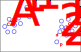
\includegraphics[width=0.5\columnwidth]{graphics/clu_kmeans_intuition.pdf}}
\caption{Intuition of K-Means clustering technique.}
\label{fig_kmeans_intuition}
\end{figure}

The K-Means technique does not specify the number of clusters in the data. This is an information that must be given as an input to the problem. However, this information is usually not known beforehand, and figuring out how many clusters the underlying patterns in the data present is actually part of what is expected of a data clustering procedure. The Principal Component Analysis, presented in the next session, comes into play in this task by facilitating that humans apply their expertise to identify patterns visually.

\subsubsection{Principal Component Analysis}

Principal Component Analysis is a data dimensionality reduction technique widely used to represent data with more than three dimensions in a graphical way in two or three dimensions. This enables humans to use their sense of vision to try to find insights in the data.

The intuition behind this technique can be explained as applying a change of basis in the data, where this new base is composed of vectors that point in the directions of maximum variance in the data. These vectors, also called Principal Components, are hierarchically sorted based on how much of the total data variance they explain.

Such principal component vectors are equivalent to the eigenvectors of the data's covariance matrix, and the variance explained by them is directly related to their associated eigenvalues \cite{b7}. Thus, the math behind PCA can be summarized by building a linear transformation matrix with the eigenvectors of the covariance matrix and then applying this linear transformation to the data in question.

The data's covariance matrix $C$, of dimensions $m \times m$, where $m$ is given as per Equation \ref{eq_pca_covmatrix}:

\begin{equation}
	\label{eq_pca_covmatrix}
	C=\frac{1}{m}\sum_{i = 1}^{m}(x^{(i)}-\mu)(x^{(i)}-\mu)^{T}   
\end{equation}




% ===============================================================
\subsection{Anomaly Detection}
\label{sec_anomaly_detection}
Anomaly Detection (AD) is a term used to refer to a number of mathematical techniques which aim to detect outliers in datasets.

These techniques can be summarized in two basic pillars:

\begin{enumerate}
	\item Providing a mathematical model that captures the underlying patterns in a dataset
	\item Using this model to declare if a given datapoint conforms to the model-associated pattern or not, that is, if it is a normal or an anomalous point
\end{enumerate}



\subsubsection{The Multi-Variate Gaussian Distribution}

The Multi-Variate Gaussian Distribution is an extension of the Gaussian Distribution in which the data-points have more than one dimension, in addition to taking to account the correlation of the variables in the dataset for the determination of the probability that the point belongs to the distribution.

This calculation is based on the covariance matrix $C$, already presented in Equation \ref{eq_pca_covmatrix}. The data-point's probability is given by Equation \ref{eq_mvg_mvg}:

\begin{equation}
	\label{eq_mvg_mvg}
	p(x|\mu,C)=\frac{1}{(2\pi)^{n/2}|C|^{1/2}}\exp{\left(\frac{1}{2}(x-\mu)^{T}C^{-1}(x-\mu)\right) }
\end{equation}

By application of Equation \ref{eq_mvg_mvg}, the "normality level" of a given observation can be directly associated with the resulting probability.

For applications in, for example, quality control, an AD technique can be implemented by simply applying a threshold to each sample's probability level and rejecting the ones below the threshold.

For vibration-based predictive maintenance, however, it is more useful to observe the variation of the vibration measurements probability over time. This approach gives then an indication of deterioration of the machine's health over time.

In order to better understand the usefulness of the MVGD, we can make use of Figure \ref{fig_mvg_singlecaseinnadequade}. A visual inspection of the Figure easily leads to the conclusion that point $x_{anom}$ does not conform to the pattern displayed by the other points, i.e., $x_{anom}$ represents an anomaly. By analysing $x_{anom}$'s coordinates $x_{1}$ and $x_{2}$ individually, the anomaly is not evident, as the coordinates are well within the range defined by the other points. By taking the correlation between $x_{1}$ and $x_{2}$ into account by means of the distribution's covariance matrix, the MVGD will then associate to $x_{anom}$ a much lower probability than for the other points, and therefore it can easily be segregated as an anomaly.

\begin{figure}[htbp]
\centerline{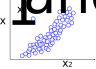
\includegraphics[width=0.5\columnwidth]{graphics/single_variab_innadequate.pdf}}
\caption{Illustration of anomaly that single variate gaussian anomaly detection strategy fails to detect.}
\label{fig_mvg_singlecaseinnadequade}
\end{figure}

A caveat when it comes to the application of the MVGD for a given dataset is the fact that it can only give meaningful results if all the dimmensions of the dataset are gaussian-distributed. Dimmensions which present high difference between mean and median, for example, are not suitable for MVGD. When such is the case, however, it is possible to apply statistical transforms to map the original distribution to another one which is more gaussian-shaped. One of such transforms is the Quantile Transform, which uses the quantile regression technique to estimate the gaussian cumulative distribution of the variable \cite{koenker2001quantile}.


% ===============================================================
% ===============================================================
% ===============================================================
\section{Hardware implementation - Data aquisition setup}
\label{sec_implementation}

The vibration monitoring hardware and software infrastructure used in this work was developed by the company DELTA Systems and is installed in a textile manufacturing plant in the city of Malatya in Turkey.

The hardware setup consists in a set of 85 wireless vibration sensors, which are all installed in a same machine and communicate with 2 gateways over radio. Figure \ref{fig_sensor_on_machine} depicts one of the sensors attached to the referred machine.

\begin{figure}[htbp]
\centerline{\includegraphics[width=8cm]{graphics/delta/sensors_machine.png}}
\caption{Textile machine with electronic sensor attached (Source: DELTA Systems GbR).}
\label{fig_sensor_on_machine}
\end{figure}


The wireless electronic sensors are embedded systems controlled by a microcontroller. The microcontroller program is written in C language, and the compiled machine code is stored in the microcontroller itself. The system also comprises an external flash memory used to store vibration measurements for later analysis and/or transmission.

An important challenge related to the operation of the sensors is their energy autonomy. Due to the small form factor of their sensors, the space available for their battery supply is limited, so that the sensor operation, defined by their firmware application code, must ensure that energy-intensive operations, such as the radio communication, are used as seldom as possible.

The gateway modules are embedded computers with a linux operational system. They run an application written in Python, which is responsible for interacting with a SQLite database, communicating with the field sensors over radio, and also providing a graphical user interface which can be accessed via TCP/IP based connection from a desktop computer connected to the same network.

An overview of this hardware, firmware and software infrastructure available to the vibration monitoring setup is depicted in Figure \ref{concept_pre}.


\begin{figure}[htbp]
\centerline{\includegraphics[width=\columnwidth]{graphics/concept/concept_pre.pdf}}
\caption{Overview of the system's architecture.}
\label{concept_pre}
\end{figure}







% ===============================================================
% ===============================================================
% ===============================================================
\section{Results and discussion}
\label{sec_results_discussion}


% ===============================================================
\subsection{Data Exploration - Overview of the vibration measurements}

The electronic sensors provide vibration measurements along the three cartesian axes $x$, $y$ and $z$, with origin and orientation assossiated to the package of the digital vibration transducer integrated circuit. By letting the fictional axis $a$ be defined as $a = \sqrt{x^{2}+y^{2}+z^{2}}$. This fictional axis $a$ then contains all the frequency components found in $x$, $y$ and $z$.

On the firmware side, the vibration measurements are configured to a sampling frequency of 4500Hz and duration of 2s. Hence, the number of samples for each axis in a measurement is $N=4500Hz \cdot 2s = 9000$. The frequency resolution resulting from an FT is, then $\Delta f + 4500Hz/9000 = 0.5 Hz$ (see Equation \ref{eq_freq_resolution}).

In Figure \ref{fig_example_signals} we can see an example of a vibration signal, on both time and frequency domain, for axes $x$, $y$, $z$ and $a$.

\begin{figure}[htbp]
\centerline{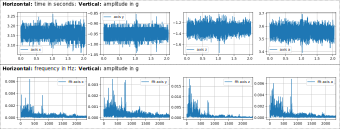
\includegraphics[width=\columnwidth]{graphics/axes_time_fft/axes_time_fft.pdf}}
\caption{Plot of an example of a vibration signal over axes $x$, $y$, $z$ and $a$, on both time (top) and frequency (bottom) domain.}
\label{fig_example_signals}
\end{figure}


% ===============================================================
\subsection{Machine speed}
\label{sec_machine_speed}

In order to obtain from the vibration measurements an indication of the speed the machine was operated at the time of the measurement, we look more closely into the frequency range from 25 to 35 Hz. As explained in Secion \ref{sec_vibration_analysis}, this region should contain the frequency related to the rotating speed of an electric motor being operated at 60Hz, which is the case of the textile machine dealth with in this work. A plot for this specific region for different $a$-axis measurement signals is presented in Figure \ref{fig_motor_frequency}. An analysis of this plot indicates that, in this range, there is sometimes indeed a peak near 30 Hz, and sometimes there is no discernible peak at all. 

An important takeaway from this observation is the confirmation that the rotating frequancy of the motor, which we from now on call $f_{motor}$, can indeed be obtained in the 25 to 35 Hz range, which allows us to restrict the costly FT calculations to this range. This means that, in the FT computations in Equation \ref{eq_fourier_disc}, the calculations are performed only for the $k$-indexes from $25Hz/\Delta f = 50$ to $35Hz/\Delta f = 70$.

As for the measurements with no discernible peak in the observed region, they presumably represent measurements acquired when the machine was not operating, as will be explained in more detail in Section \ref{sec_clustering_results}.

\begin{figure}[htbp]
\centerline{\includegraphics[width=\columnwidth]{graphics/motor_frequency/motor_frequency.pdf}}
\caption{Observations of the $a$-axis frequency spectra in the expected range for $f_{motor}$.}
\label{fig_motor_frequency}
\end{figure}



% ===============================================================
\subsection{Digital Filters}

In the introduction to Section \ref{sec_signal_processing} we presented three vibration signal characteristics of interest for our analysis. 

The first of them, the machine's speed, can be represented by $f_{motor}$, obtained as explained in Section \ref{sec_machine_speed}. 

The second one, the energy content of the vibration signal, can be easily obtained by the RMS value of the $a$-axis of the measurement.

In this section, we detail how to obtain the third and last one: the distribution of the vibration's energy over its frequency spectrum. As already explained in Section \ref{sec_digital_filters_concept}, this can be acomplished with reasonable computational cost by computing the RMS values of the output of digitail filters.

For this purpose, the available frequency range of up to 2250 Hz is divided into three ranges:

\begin{itemize}
	\item a lower range up to 500 Hz
	\item a middle range betwen 500 and 1250 Hz
	\item a higher range from 1250 Hz on
\end{itemize}

The higher the number of ranges, the more detailed the vibration energy distribution over frequency, at the cost of more computations required.

For each of these ranges, a digital filter was developed. These filters are then named $F_{low}$, $F_{mid}$ and $F_{high}$, acording to their associated frequency range.

By taking to account the discussion in Section \ref{sec_digital_filters_concept}, the main design decisions are summarized as follow:

\begin{itemize}
	\item Topology: The topology chosen was the inverse Chebyshev. The first reason for this choice is the narrow transition band, which is always desirable. The tradeoff for the narrower transition band is a larger phase distortion, which is irrelevant
	for our case, as we do not take phase into account in our modelling. Finally, we desired a flat passband in order to preserve as much as possible the information of the passband for our modelling.
	\item Order: As a general rule, the overall performance of the filter is improved with higher order, at the cost of more computations required. By experimentation, the	order value was set to 3.
	\item Overlap: Some overlap was included in the cutoff frequencies of the three filters. This was a decision taken in orther to achieve an optimum configuration within the numerous tradeoffs in filter design. Hence, $F_{low}$ was defined as a low-pass with cuttoff at 700 Hz, $F_{mid}$ was defined as a band-pass with cutoffs at 400 and 1350 Hz, and $F_{high}$ as a high-pass at 1150 Hz.
\end{itemize}

The frequency response of the three filters is presented in \ref{fig_filters_freq_response}. Figure \ref{fig_filters_example_inout} depicts the output of the filters, in time and frequency domain, for an example $a$-axis measurement input signal.

\begin{figure}[htbp]
\centerline{\includegraphics[width=\columnwidth]{graphics/filters_freqresponse/filters_freqresponse.pdf}}
\caption{Frequency response of the three filters.}
\label{fig_filters_freq_response}
\end{figure}

\begin{figure}[htbp]
\centerline{\includegraphics[width=\columnwidth]{graphics/filters_sigresponse/filters_sigresponse.pdf}}
\caption{Filters, in time and frequency domain, for an example $a$-axis measurement input signal.}
\label{fig_filters_example_inout}
\end{figure}



% ===============================================================
\subsection{Clustering: Segregation of Operational Modes}
\label{sec_clustering_results}


In order to understand the underlying patterns in the data, the first step was to carry out a Principal Component Analysis on the dataset. The input to this analysis contained five features:

\begin{itemize}
	\item $f_{motor}$: peak frequency in the 25Hz to 35 Hz range
	\item $RMS_{total}$: RMS value of the $a$ axis
	\item $RMS_{low}$: RMS value of the output of the $f_{low}$ filter
	\item $RMS_{mid}$: RMS value of the output of the $f_{mid}$ filter
	\item $RMS_{high}$: RMS value of the output of the $f_{high}$ filter
\end{itemize}

The resulting PCA plot is presented in \ref{fig_pca_result}. This same plot also shows a seggregation of the points based on the results of a Kmeans clustering procedure.


\begin{figure}[htbp]
\centerline{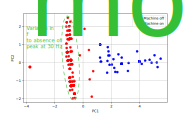
\includegraphics[width=\columnwidth]{graphics/pca_result/pca_result.pdf}}
\caption{PCA plot for the described dataset}
\label{fig_pca_result}
\end{figure}

While analysing the measurements assigned to each cluster, it was noted that one of the clusters was characterised by lower vibration levels in general than the other one. This lead to the conclusion that the former represents the "operational" state for when the machine is off, and the later for when the machine is on. This conclusion is supported by the region with large variation, encircled in a green dashed shape. When the machine is off, the motors are not running, so they do not produce the 30 Hz peak, thus the peak in the 25 Hz to 35 Hz range ends up being mostly randomly defined by noise.

When the machine is off, its vibration signature is of low relevance for PM. Thus, the analysis from this point on focuses on the cluster that represents the machine in its "on" state. The segregation can be easily carried out by thresholding the $RMS_{total}$ value. This threshold value was set to $0.015g$. It is worth at this point to recap that the $a$ axis signal has its average value removed, so the $1g$ gravity vibration is not present in the signal.



% ===============================================================
\subsection{Approach to Anomaly Detection}


At this point in the data analysis, the data is already clustered, and a single cluster was selected for further analysis. Thus, the variability left in the data is expected not to result in multimodal distributions for a given variable. In order to implement the multi-variate Gaussian distribution AD strategy discussed in \ref{sec_anomaly_detection}, it is required that the variables are Gaussian-distributed. In order to make sure this is the case, we apply a normalization transform to the data unsing the quantile transform described in the same Section.

Figure \ref{fig_transform_result} depicts the variables before and after the transformation.

% \begin{figure}
% 	\centering
% 	\includegraphics[width = \textwidth]{quantile_transform_data/quantile_transform_data.pdf}
% 	\caption[Transformed data]{Variables before and after quantile transform}
% 	\label{fig_transform_result}
% \end{figure}

\begin{figure}[htbp]
\centerline{\includegraphics[width=\columnwidth]{graphics/quantile_transform_data/quantile_transform_data.pdf}}
\caption{Variables before and after quantile transform}
\label{fig_transform_result}
\end{figure}


Then, for the actual AD approach, it was decided to build a concept based on the evaluation of the MVGD probability for four distinct models:

\begin{enumerate}
	\item Covariance between $f_{motor}$ and $RMS_{total}$
	\item Covariance between $f_{motor}$, $RMS_{total}$ and $RMS_{low}$
	\item Covariance between $f_{motor}$, $RMS_{total}$ and $RMS_{mid}$
	\item Covariance between $f_{motor}$, $RMS_{total}$ and $RMS_{high}$
\end{enumerate}


Figure \ref{fig_mvgd_plot1} represents the measurement points associated probability given the covariance model $(f_{motor},RMS_{total})$. In this 3D heatmap representation, the $x$ and $y$ axes represent, respectively the transformed $f_{motor}$ and $RMS_{total}$ variables, while the resulting $z$ axis, like the associated heatmap color, represent the measurement point's assiciated probability.

% \begin{figure}
% 	\centering
% 	\includegraphics[width = \textwidth]{mvgd_plots/plot1_fmotor_rmstotal.pdf}
% 	\caption[MVGD plot for $f_{motor}$ and $RMS_{total}$]{MVGD plot for $f_{motor}$ and $RMS_{total}$}
% 	\label{fig_mvgd_plot1}
% \end{figure}

\begin{figure}[htbp]
\centerline{\includegraphics[width=\columnwidth]{graphics/mvgd_plots/plot1_fmotor_rmstotal.pdf}}
\caption{MVGD plot for $f_{motor}$ and $RMS_{total}$}
\label{fig_mvgd_plot1}
\end{figure}

The "normality" values for the four covariance models designed are then tracked over time in days in \ref{fig_controlchart_all}. As it can be seen in the plots, it is, unfortunately, not possible to establish a significant deterioration trend or any clearly alarming anomaly. The main cause for this problem is the fact that there are long periods of time without available measurements. With additional data regularly aquired, it should be possible to detect trends more clearly.


% \begin{figure}
% 	\centering
% 	\includegraphics[width =\textwidth]{control_charts/control_chart_v02.pdf}
% 	\caption[Time-evolution of the "normality" values]{Time-evolution of the "normality" values for the different covariance models designed }
% 	\label{fig_controlchart_all}
% \end{figure}

\begin{figure}[htbp]
\centerline{\includegraphics[width=\columnwidth]{graphics/control_charts/control_chart_v02.pdf}}
\caption{Time-evolution of the "normality" values for the different covariance models designed}
\label{fig_controlchart_all}
\end{figure}


% ===============================================================
\subsection{System Update - Increasing Sensor Throughput}

One of the causes for the periods of time without data in Figure \ref{fig_controlchart_all} is due to the battery of the sensors being depleted. The main consumer of battery energy in the sensors is the radio module. Hence, transmitting less data directly results in less power consumption and thus to longer battery life.

In the current system FW and SW, the sensors send the measurement signals entirelly. However, by optimized implementations of the Fourier Transform and Digital Filtering techniques exposed here, the sensor is able to extract the desired features from the measurement data by itself and then send only the features by radio. Through lab experiments, the energy required to send all the data for a measurement is $E_{alldata}\approx 3.64 Ws$, while the energy required to extract the features with the signal processing techniques described and sending only the desired features is $E_{sigprocess} \approx 0.51 Ws$. The energy reduction per measurement achieved is then $E_{longmm}/E_{sigprocess} \approx 7.14$.

The new sensor FW, with the optimized signal processing techniques for feature extraction, is to be included in next stages of the vibration monitoring project as a whole in the textile manufacturer's site.






% ===============================================================
\subsection{The Way to the Internet of Things}
The efforts dedicated to this work are considered the preparation of a decentralized connection to an Internet of Things. From the view of the vibration system, it is meaningful to employ global connectivity since, without it, the system is only available and accessible across the local network consisting of the textile machine and the edge device.

The deployment of the 	IoT network should cover, apart from the connectivity, the communication security according to the CIA (confidentiality, integrity, and availability) Triad and AAA (authentication, authorization, and accounting) model, user privacy, and interoperability with defined semantics. The utilization of security measurements, in combination with the edge-based approach, is able to ensure the self-sovereign of monitored data, as it is never hosted in a public cloud, and access to it is carefully restricted.


% ===============================================================
% ===============================================================
% ===============================================================
\section{Conclusion}
\label{sec_conclusion}

% ===============================================================
% ===============================================================
% ===============================================================
\section*{Acknowledgment}
The authors thank Mr. Georg Sommer, software engineer at DELTA Systems GbR, for his work in writing the gateway's software infrastructure which enabled the aquisition, storage and retrieval of the data produced by the electronic sensors.

% ===============================================================
% ===============================================================
% ===============================================================
% \section*{References}


\begin{thebibliography}{00}

	\bibitem{b1} R. B. Randall, ``Vibration-based condition monitoring: industrial, automotive and aerospace applications,'' John Wiley \& Sons, 2021.


    \bibitem{b2} M. Tsypkin, ``The Origin of the Electromagnetic Vibration of Induction Motors Operating in Modern Industry: Practical Experience—Analysis and Diagnostics,'' IEEE Transactions on Industry Applications, vol. 53, pp. 1669--1676,2017.


    \bibitem{b3} H. P. Bloch and F. K. Geitner, ``Machinery Failure Analysis and Troubleshooting: Practical Machinery Management for Process Plants,'' Elsevier, 2012.


    \bibitem{b4} L. Tan and J. Jiang, ``Digital signal processing: fundamentals and applications,'' Academic Press, 2018.


    \bibitem{b5} A. J. Jerri, ``The Shannon sampling theorem—Its various extensions and applications: A tutorial review,'' Proceedings of the IEEE, vol. 65, pp. 1565--1596, 1877.

	\bibitem{b7} M. E. Wall and A. Rechsteiner and L. M. Rocha, ``Singular value decomposition and principal component analysis,'' in ``A practical approach to microarray data analysis,'' p91--109, Springer, 2003.


	\bibitem{koenker2001quantile} R. Koenker and K. F. Hallock, ``Quantile regression,'' in ``Journal of economic perspectives,'' p143--156, vol 15, 2001.




	\bibitem{carnero2006evaluation} M. Carnero, ``An evaluation system of the setting up of predictive maintenance programmes,'' in ``Reliability Engineering \& System Safety,'' p945--963, vol 91, Elsevier,2006.
	
	\bibitem{wu2017remaining} B. Wu and W. Li and M. Qiu, ``Remaining useful life prediction of bearing with vibration signals based on a novel indicator,'' in ``Shock and Vibration,'' Hindawi, 2017.
	
	\bibitem{li2020lifelong} C. Li, and L. Mo and H. Tang and R. Yan, ``Lifelong Condition Monitoring Based on NB-IoT for Anomaly Detection of Machinery Equipment,'' in ``Procedia Manufacturing,'' p144--149, vol 49, Elsevier, 2020.
	
	\bibitem{cui2018anomaly} Y. Cui and P. Bangalore and L. B. Tjernberg, ``An anomaly detection approach using wavelet transform and artificial neural networks for condition monitoring of wind turbines' gearboxes,'' in ``2018 Power Systems Computation Conference (PSCC),'' p1--7, IEEE, 2018.

	\bibitem{adebiyi} K. A. Adebiyi and J. O. Ojediran and O. A. Oyenuga, ``An appraisal of maintenance practice in food industries in Nigeria,'' in ``Journal of Food Engineering,'' p131--133, vol 62, Elsevier, 2004.

	\bibitem{alnajjar} B. Al-Najjar and I. Alsyouf, ``Enhancing a company's profitability and competitiveness using integrated vibration-based maintenance: A case study,'' in ``European Journal of Operational Research,'' p643--657, vol 157, Elsevier, 2004.

	\bibitem{doyleek} E. K. Doyle, ``On the application of stochastic models in nuclear power plant maintenance,'' in ``European Journal of Operational Research,'' p673--60, vol 154, Elsevier, 2004.

	\bibitem{doyleek} K. E. Chong and K. C. Ng and G. G. G. Goh, ``OImproving Overall Equipment Effectiveness (OEE) through integration of Maintenance Failure Mode and Effect Analysis (maintenance-FMEA) in a semiconductor manufacturer: A case study,'' in ``2015 IEEE International Conference on Industrial Engineering and Engineering Management (IEEM),'' p1427--1431, Elsevier, 2015.
	
\end{thebibliography}

\end{document}
